\documentclass[border=0pt]{standalone}

\usepackage{tikz}        % drawing macros
  \usetikzlibrary{math}
  \usetikzlibrary{calc}  % calculations
  \usetikzlibrary{arrows}  % arrowheads
  \usetikzlibrary{arrows.meta}  % arrowheads
  \usetikzlibrary{decorations.markings}
\usepackage{tikz-3dplot} % drawing macros 3d
\usepackage{pgfplots}
%\pgfplotsset{compat=1.18}

\begin{document}

\resizebox{!}{1.0in}{

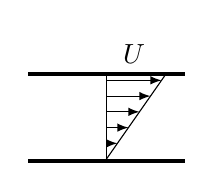
\begin{tikzpicture}
\tikzset{>=latex}

% Bottom wall
  \coordinate (B1) at (-1.00, 0.00);
  \coordinate (B2) at ( 1.00, 0.00);
  \coordinate (B3) at ( 1.00,-0.05);
  \coordinate (B4) at (-1.00,-0.05);
  \fill[thick] (B1) -- (B2) -- (B3) -- (B4) -- cycle;

% Top wall
  \coordinate (T1) at (-1.00, 1.05);
  \coordinate (T2) at ( 1.00, 1.05);
  \coordinate (T3) at ( 1.00, 1.10);
  \coordinate (T4) at (-1.00, 1.10);
  \fill[thick] (T1) -- (T2) -- (T3) -- (T4) -- cycle;

% Profile
  \draw     (0.00,0.00) -- +(0.00,1.10);
  \draw     (0.00,0.00) -- +(0.77,1.10);
  \draw[->] (0.00,0.20) -- +(0.14,0.00);
  \draw[->] (0.00,0.40) -- +(0.28,0.00);
  \draw[->] (0.00,0.60) -- +(0.42,0.00);
  \draw[->] (0.00,0.80) -- +(0.56,0.00);
  \draw[->] (0.00,1.00) -- +(0.70,0.00) node[midway,above,inner sep=6pt] {$U$};

\end{tikzpicture}

} % end \resizebox

\end{document}
